\graphicspath{ {images/} }
\chapter{Design}
\hspace{5mm} In previous chapter when you finished literature to understand methods.Their may be many methods to develop your proposed system.But one which you chose to implement that need to be design in this chapter.


\section{Architecure}
\hspace{5mm}This part contain architecture(figure) which can be either flow design or analytic model or mathematical model or any other design.
\par database design also included in this part.
\\
\begin{figure}[h!]
\begin{center}
\scalebox{1.30}{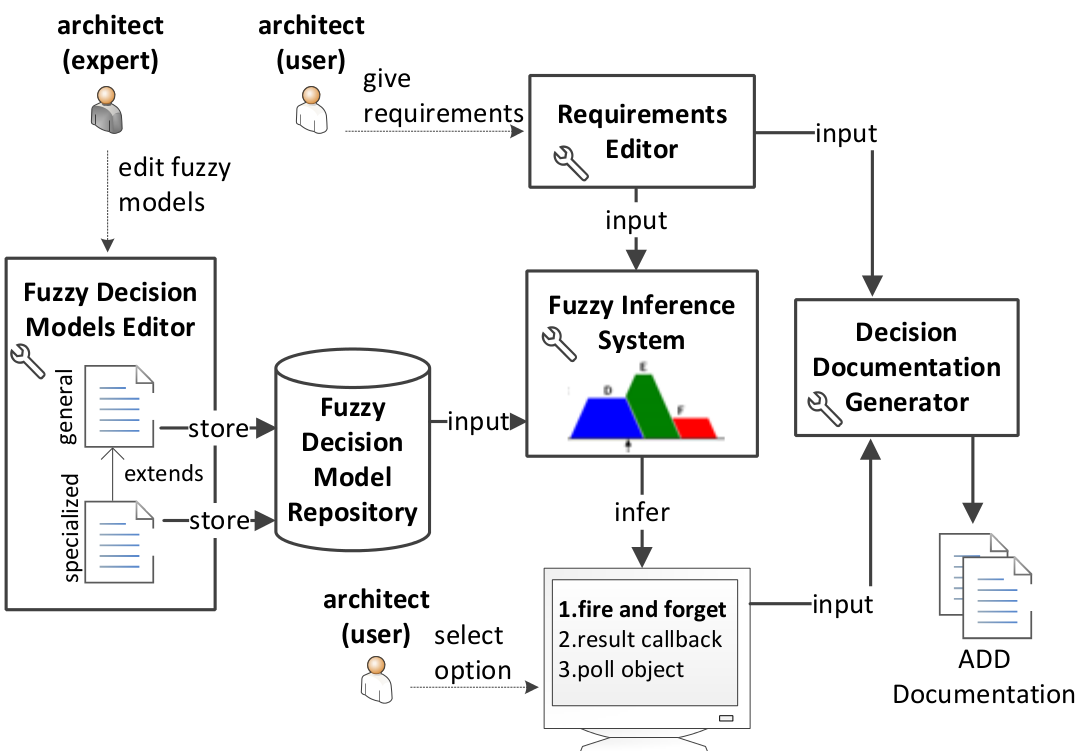
\includegraphics{images/architecture.png}}
\end{center}
\caption {System Architecture}
\label{vmb2}
\vspace{0mm}
\end{figure}

\par here you can explain which methodology you followed for your project through designs.Explain every block from architecture.
\begin{itemize}
    \item \textbf{Block1:} Ability to enforce uniform enterprise authentication and/or authorization policies across the enterprise
    \item \textbf{Block2:} End to end user audit sessions to improve security reporting and auditing
    \item \textbf{Block3:} Removes application developers from having to understand and implement identity security in their applications
    \item \textbf{Block4:} Usually results in significant password help desk cost savings
\end{itemize}

\section{Detailed Design}
\hspace{5mm}In this section you need to put diagram/figures related to detailed design like UML diagrams. Also give small description about every diagram.(Must take suggestion from guide)  
\\
\begin{figure}[h!]
\begin{center}
\scalebox{0.50}{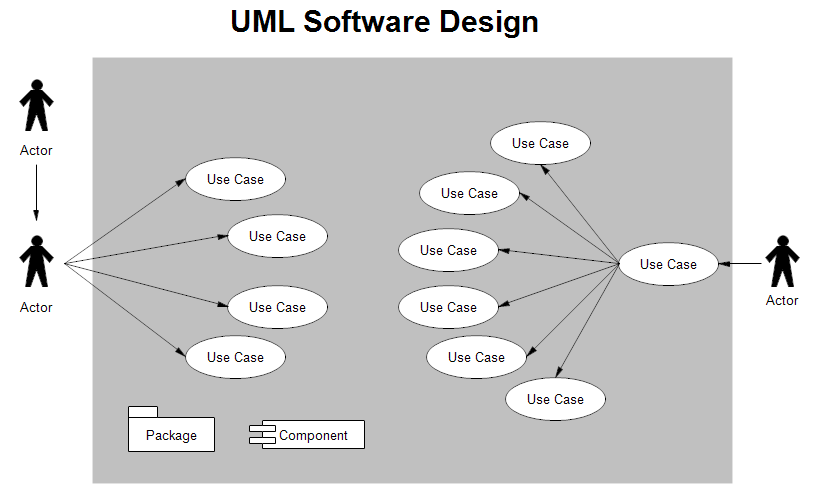
\includegraphics{images/usecase.png}}
\end{center}
\caption {use case}
\label{vmb2}
\vspace{0mm}
\end{figure}

\hspace{5mm}Small description about above diagram.

\begin{figure}[h!]
\begin{center}
\scalebox{1.00}{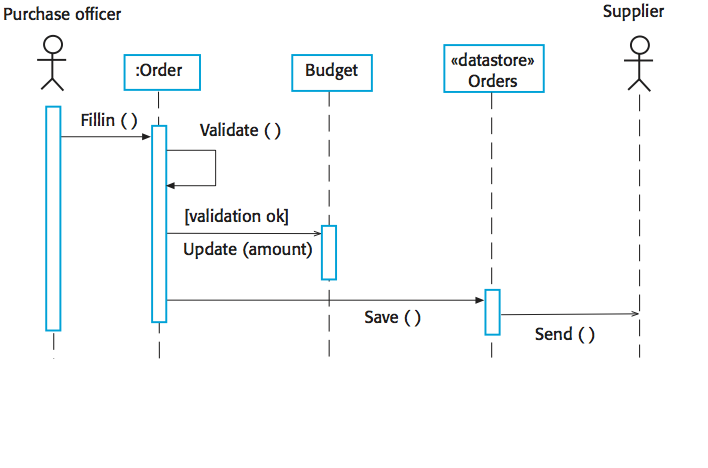
\includegraphics{images/sequence.png}}
\end{center}
\caption {Sequence Diagram}
\label{vmb2}
\vspace{0mm}
\end{figure}

\hspace{5mm}Small description about above diagram.

